\documentclass[prb,twocolumn,9pt]{revtex4-1}

% LOAD PACKAGES

% GENERAL PACKAGES
\usepackage{graphicx}
\usepackage{wrapfig}
\usepackage{color}
\usepackage{latexsym,amsmath}
\usepackage{physics}
\usepackage{chemformula}
\usepackage{tabularx}
\usepackage{float}
\usepackage{siunitx}
\usepackage{amssymb}
%\usepackage[caption=false, justification=right]{subfig} % rovina la formattazione delle figure se caption=true
\usepackage[caption=false]{subfig}
\usepackage{multirow}

% LISTING PACKAGES
\usepackage{xcolor}
\usepackage{listings}
\usepackage{framed}
\usepackage{inconsolata} % To change the listing font

% URL PACKAGE AND SETTING
\definecolor{linkcolor}{rgb}{0,0,0.65} %hyperlink
\definecolor{linescolor}{rgb}{0.65,0.16,0.16}
\definecolor{cool}{RGB}{49,54,149}
\definecolor{hot}{RGB}{165,0,38}
\usepackage[pdftex,colorlinks=true, pdfstartview=FitV, linkcolor= linescolor, citecolor= linescolor, urlcolor= linkcolor, hyperindex=true,hyperfigures=true]{hyperref} %hyperlink%

% PAGE SETTING
\usepackage{fancyhdr} 

\pagestyle{fancyplain}
\fancyhf{}
\renewcommand{\headrulewidth}{0pt}
\fancyfoot[R]{\textbf{\thepage}}
%\fancyfoot[L]{Università degli Studi di Padova - Dipartimento di Fisica e Astronomia Galileo Galilei} 
%\fancyhead[L]{\textbf{Advanced Physics Laboratory Report}}
%\fancyhead[L]{\ifnum\value{section}>0\nouppercase{\textbf{\leftmark}\fi}}
%\fancyhead[R]{\textbf{Name1 Surname1 - Name2 Surname2}}
%\renewcommand{\headrulewidth}{0.2pt}
%\renewcommand{\footrulewidth}{0.1pt}

%\setlength\parindent{9pt} % To adjust the intendation

% SECTION STYLE
%Redefine \thesubsection as \thesection.\alph{subsection}. (\alph replaces the default \arabic; you could also choose, e.g., \Alph, \roman, and \Roman.)
\renewcommand{\thesection}{\textbf{\Roman{section}}}
\renewcommand{\thesubsection}{\textbf{\arabic{subsection}}}
\renewcommand{\thesubsubsection}{\textbf{\Alph{subsubsection}}}
%\renewcommand{\thesection}{\textbf{\arabic{section}}}
%\renewcommand{\thesubsection}{\thesection.\textbf{\arabic{subsection}}}
%\renewcommand{\thesubsubsection}{\textbf{\thesection.\arabic{subsection}.\arabic{subsubsection}}}

% FIGURE AND TABLE STYLE
\renewcommand{\tablename}{\textbf{TAB.}}
\renewcommand{\thetable}{\textbf{\arabic{table}}}

% ELIMINARE COMMENTO NELLA COMPILAZIONE FINALE
%\renewcommand{\figurename}{\textbf{FIG.}}
%\renewcommand{\thefigure}{\textbf{\arabic{figure}}}

% BIBLIOGRAPHY FILE AND SETTING
\bibliographystyle{aipnum4-1}
\setcitestyle{numbers,square}

%\usepackage[backend=biber, sorting=ynt]{biblatex}
%\addbibresource{references.bib}


\begin{document}



% FRONTESPIZIO

% Title
\title{Insert Title Here}



\author{Alice Pagano}


\date{\today}

% Abstract
\begin{abstract}

Insert abstract here

\end{abstract}


% Make title
\maketitle



\section{Introduction}
\label{sec:introduction}

In the last months, in particular after....


% \begin{table}[b]
%    \begin{minipage}[l]{1.0\columnwidth}
%    \centering
%        \begin{tabular*}{\linewidth}{@{\extracolsep{\fill}}
%        l cccc 
%        }
%       %\toprule
%            & \textbf{2017} & \textbf{2018} &  \textbf{2019} & \textbf{2020} \\
%        \colrule
%            $\pmb{d_t}$    & 438 & 405 & 382 & 277 \\
%       % \colrule
%            $\pmb{d_{nv}}$ & 83.3 \% & 88.6 \% & 98.2 \% & 82.3 \% \\
%       % \colrule
%            $\pmb{d_{u}}$  & 22.5 \% & 32.3 \% & 39.2 \% & 59.2 \% \\
%       %\botrule
%        \end{tabular*}
%    \caption{Dataset dimension for the different years under study. $d_t$ is the total dimension of the tweet dataset after location classification. $d_{nv}$ is the percentage of $d_t$ of tweets that express actually a novax opinion. $d_u$ is the percentage of unique users of $d_{nv}$. }
%    \label{tab:dataset_dimension}
%    \end{minipage}
%    \end{table}
    

%\begin{figure}[t]
%   \begin{minipage}[l]{1.0\columnwidth}
%   \centering
%   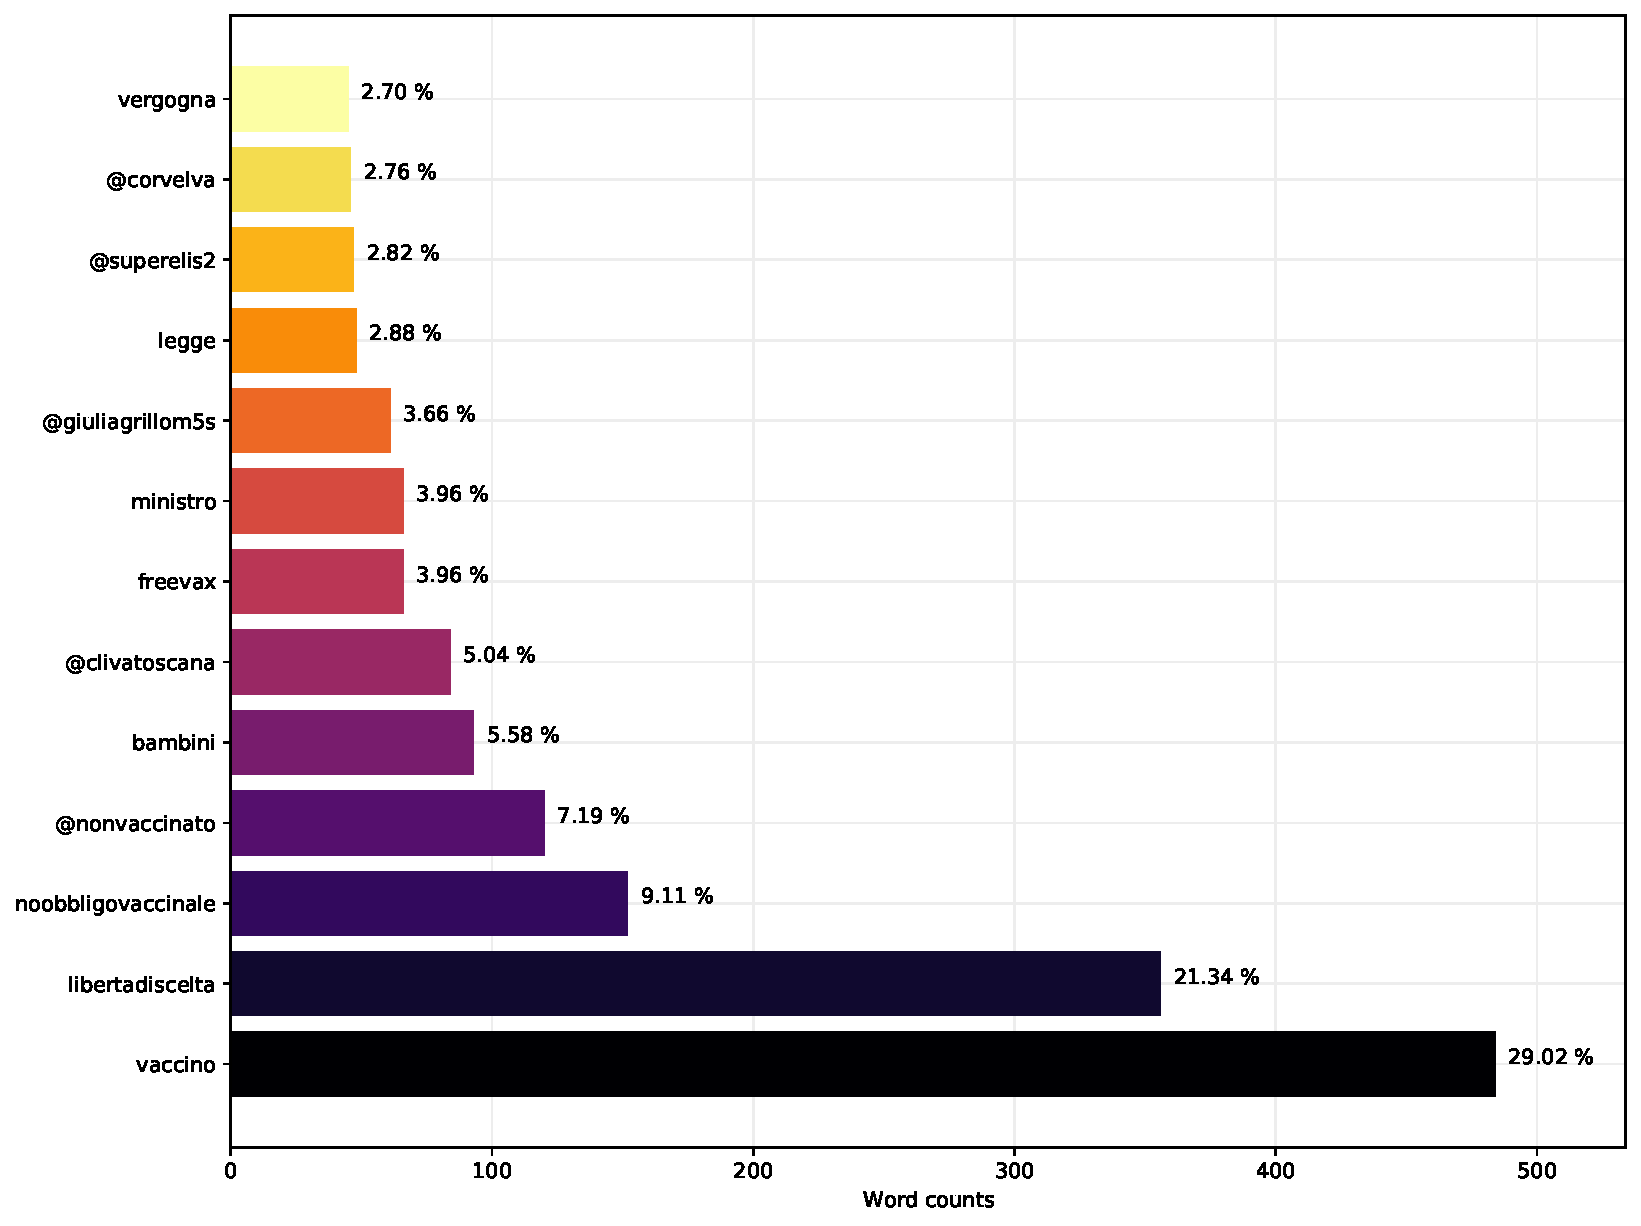
\includegraphics[width=1\textwidth]{Paper_template/image/word_2017-2020.pdf}
%   \caption{Histogram of most used words in the novax collected tweets in 2017-2020 time interval.}
%   \label{fig:count_word}
%   \end{minipage}
%\end{figure}

% \begin{table}[b]
%    \begin{minipage}[l]{1.0\columnwidth}
%    \centering
%        \begin{tabular*}{\linewidth}{@{\extracolsep{\fill}} c c c c}
%       \textbf{Region}	&	\textbf{$I$}	&	\textbf{$A$} &	\textbf{$\frac{I- A}{I}$}	\\
% \colrule
%Prov. Au. di Bolzano	&	0.9	&	0.2	&	0.7	\\
%Molise	&	0.5	&	0.2	&	0.6	\\
%Sicilia	&	8.2	&	5.5	&	0.3	\\
%Puglia	&	6.6	&	4.5	&	0.3	\\
%Prov. Au. di Trento	&	0.9	&	0.6	&	0.3	\\
%Calabria	&	3.2	&	2.3	&	0.3	\\
%Campania	&	9.6	&	7.3	&	0.2	\\
%Basilicata	&	0.9	&	0.7	&	0.2	\\
%Friuli Venezia Giulia	&	2.0	&	1.6	&	0.2	\\
%Veneto	&	8.2	&	6.6	&	0.2	\\
%Abruzzo	&	2.2	&	1.8	&	0.2	\\
%Sardegna	&	2.7	&	2.4	&	0.1	\\
%Valle d'Aosta	&	0.2	&	0.2	&	0.1	\\
%Piemonte	&	7.2	&	7.1	&	0.0	\\
%Umbria	&	1.5	&	1.5	&	0.0	\\
%Marche	&	2.5	&	2.7	&	-0.1	\\
%Emilia Romagna	&	7.5	&	8.5	&	-0.1	\\
%Lombardia	&	16.8	&	19.2	&	-0.1	\\
%Toscana	&	6.2	&	7.5	&	-0.2	\\
%Liguria	&	2.6	&	3.4	&	-0.3	\\
%Lazio	&	9.7	&	16.0	&	-0.7	\\
%
%        \end{tabular*}
%    \caption{Percentage of inhabitants $I$ (at 1 January 2020 \cite{istat}) and Twitter activity $A$ of the Italian regions. Data are sorted in descending order according to the third column $\frac{I- A}{I}$ which quantifies how active a region is on Twitter compared to the number of inhabitants.}
%    \label{tab:inhab-activity}
%    \end{minipage}
%    \end{table}

%	% To insert four subfigure
%	\begin{figure*}[t]
%	\begin{minipage}[c]{0.49\linewidth}
%	\centering
%	\subfloat[][2017]{\includegraphics[width=0.8\textwidth]{Paper_template/image/map/map_2017.pdf} \label{fig:map_result_a} }
%	\end{minipage}
%	\begin{minipage}[]{0.49\linewidth}
%	\centering
%	\subfloat[][2018]{\includegraphics[width=0.8\textwidth]{Paper_template/image/map/map_2018.pdf} \label{fig:map_result_b} }
%	\end{minipage} \\
%	\vfill
%	\begin{minipage}[c]{0.49\linewidth}
%	\centering
%	\subfloat[][2019]{\includegraphics[width=0.8\textwidth]{Paper_template/image/map/map_2019.pdf} \label{fig:map_result_c} }
%	\end{minipage}
%	\begin{minipage}[]{0.49\linewidth}
%	\centering
%	\subfloat[][2020]{\includegraphics[width=0.8\textwidth]{Paper_template/image/map/map_2020.pdf} \label{fig:map_result_d} }
%	\end{minipage}
%	\caption{\label{fig:map_result} Superposition maps of measles vaccination coverage (shades of red) and novax activity on Twitter (blue points with radius proportional to its weight). The years under analysis are 2017-2020. Vaccination coverage for 2020 is not available, so, in 2020 map, 2019 vaccination coverage is used.}
%	\end{figure*}
    


\section{Conclusions}
\label{sec:conclusions}

In this work, we analyze the distribution...



% To add bibliography (file references.bib)
\bibliographystyle{unsrt}
\bibliography{references}{}
%\printbibliography

\end{document}
